\chapter{Senzory}
\label{sec:Sensors}
\vspace{-20pt}
\

Platforma FRDM-K66F obsahuje tří senzory, které tvoří
9-osou IMU jednotku. Konkretně jako akcelerometr a magnetometr deska má
NXP FXOS8700CQ a gyroskop NXP FXAS21002. Tyto senzory komunikují s platformou
pomocí $I^2C$\cite{frdmk66UserGuide}.

\section{NXP FXOS8700CQ}\

\textbf{NXP FXOS8700CQ} je pokročilý 6-osy senzor,
který kombinuje funkce 3-os akcelerometru
a 3-os magnetometru do jednoho čipu. Akcelerometr v senzoru FXOS8700CQ má
nastavitelné rozsahy ±2 g, ±4 g, ±8 g s 14-bitovým rozlišením, zatímco magnetometr
poskytuje 16-bitové rozlišení s rozsahem ±1200 µT na osu. Pro komunikaci podporuje
$I^2C$ a SPI rozhraní. Má dva piny pro~přerušení a podporuje odesílat data rychlosti
až 800 Hz pro každý senzor a až 400 Hz v hybridním režimu.
Tato~integrace umožňuje zařízení zachytit komplexní data o svém pohybu a
orientaci vůči zemskému gravitačnímu a magnetickému poli.
Orientace akcelerometru a magnetometru je na obrázku \ref{fig:FXOS_Orientation}
\cite{FXOS8700CQ}.

\begin{figure}[!h]
    \centering
    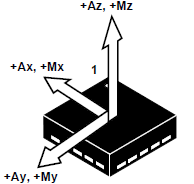
\includegraphics[width = 0.5\linewidth]{Figures/FXOS_Orientation.png}
    \caption{NXP FXOS8700CQ orientace\cite{FXOS8700CQ}.}
    \label{fig:FXOS_Orientation}
\end{figure}

\section{NXP FXAS21002}\

\textbf{NXP FXAS21002} je vysoce výkonný 3-osy senzor, který poskytuje data o úhlové rychlosti
zrychlení. Tento senzor má nastavitelné rozsahy ±250, ±500, ±1000, a
±2000 stupňů za sekundu
s 16-bitovým rozlišením. Pro komunikaci podporuje $I^2C$ a SPI rozhraní.
Má dva piny pro přerušení a podporuje odesílat data rychlosti až 800 Hz.
To umožňuje zařízení detekovat rotace kolem svych os.
Orientace gyroskopu je na obrázku \ref{fig:FXAS_Orientation}\cite{FXAS21002}.

\begin{figure}[!h]
    \centering
    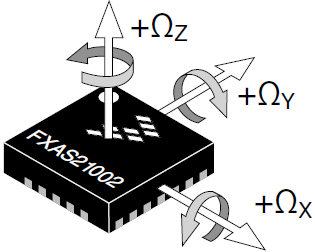
\includegraphics[width = 0.5\linewidth]{Figures/FXAS_Orientation.png}
    \caption{NXP FXAS21002 orientace\cite{FXAS21002}.}
    \label{fig:FXAS_Orientation}
\end{figure}

\section{Komunikace se senzory}\

Pro komunikaci se senzory je použito $I^2C$ sběrnice.

$I^2C$ sběrnice má 2 vodiče pro všichni zařízení, SDA a SCL.
\textbf{SDA} je datová linka, která
přenáší data mezi zařízeními, zatímco \textbf{SCL} je hodinová linka, která synchronizuje
přenos dat. Na sběrnice existuje jedno zařízení, které je master, a může komunikovat
s zařízeními, které jsou slave. \textbf{Master zařízení} generuje hodinový signál a
určuje, kdy se data posílají a přijímají. Každé zařízení na~sběrnici má svou
vlastní adresu, která je 7 bitů dlouhá. Oba vodiče jsou aktivní nízké, což znamená,
že v klidovém stavu jsou oba vodiče v logické 1. Když je zařízení připojeno k
systému, musí být připojeno k zemi, aby mohlo komunikovat.

Přenos na sběrnice vždy začíná START sekvencí a končí STOP sekvencí,
viz. obrázek \ref{fig:I2C_FRAME}. Ty jsou generovány Master zařízením.
\textbf{START} sekvence je definovaná jako přechod z logické 1 na logickou 0 na SDA, zatímco
SCL je v logické 1. \textbf{STOP} sekvence je definována jako přechod z~logické 0 na~logickou 1 na SDA, zatímco SCL je v logické 1. Sběrnice je obsazena od začátku START sekvence
až do konce STOP sekvence.

Pro zápis dat na sběrnici je nejprve nutné poslat adresu zařízení, které přijímá
data. Adresa má 7 bitů a poslední bit je R/W, který určuje, zda se jedná
o zápis nebo čtení. Poté jak Slave pošle ACK bit, což znamená, že je připraven přijmout
data, Master posílá data a Slave potvrzuje přijetí ACK bitem.

Čtení dat je podobné zápisu, ale po odeslání adresy zařízení, které posílá data,
Master přepne do režimu čtení a Slave pošle data, která Master potvrzuje ACK bitem\cite{I2C}.

\begin{figure}[!h]
    \centering
    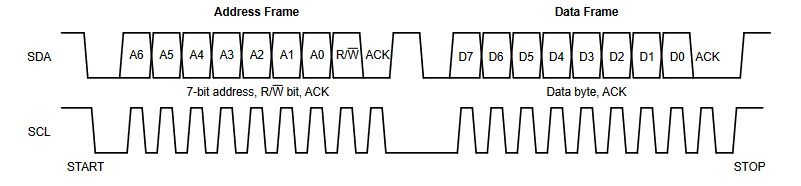
\includegraphics[width = 0.8\linewidth]{Figures/I2C_FRAME.png}
    \caption{I2C frame\cite{I2C}.}
    \label{fig:I2C_FRAME}
\end{figure}

\section{Konfigurace senzorů}\

Pro konfiguraci senzorů je nutné poslat data na jejich adresy. Adresa NXP FXOS8700CQ
je 0x1D a adresa NXP FXAS21002 je 0x21.

\subsection{Konfigurace NXP FXOS8700CQ}\

Pro nastavení NXP FXOS8700CQ bylo nastaveny nasledující registry: CTRL\_REG\_1, CTRL\_REG\_2,
CTRL\_REG\_4, CTRL\_REG\_5, M\_CTRL\_REG\_1, M\_CTRL\_REG\_2, XYZ\_DATA\_CFG.
Adresa registru a hodnoty jsou v tabulce \ref{tab:FXOS8700CQ}.

\begin{table}[!h]
    \centering
    \begin{tabular}{|c|c|c|}
        \hline
        \textbf{Adresa} & \textbf{Registr} & \textbf{Hodnota} \\
        \hline
        0x2A            & CTRL\_REG1       & 0x1D             \\
        0x2B            & CTRL\_REG2       & 0x1E             \\
        0x2D            & CTRL\_REG4       & 0x01             \\
        0x2E            & CTRL\_REG5       & 0x00             \\
        0x5B            & M\_CTRL\_REG1    & 0x5F             \\
        0x5C            & M\_CTRL\_REG2    & 0x20             \\
        0x0E            & XYZ\_DATA\_CFG   & 0x01             \\
        \hline
    \end{tabular}
    \caption{Konfigurace NXP FXOS8700CQ\cite{FXOS8700CQ}.}
    \label{tab:FXOS8700CQ}
\end{table}

Registr CTRL\_REG1 je použit pro přepnutí režimu senzoru mezi standby a active.
Pro jakekoliv změny v registrech je nutné přepnout senzor do standby režimu.
Pokud všechny registry byly nastaveny, je možné přepnout senzor do active režimu, a dále
tento registr použit pro nastavení frekvence vzorkování na 50 Hz a zapnutí malého šumu.

Registr CTRL\_REG2 je použit pro zapnutí automatického režimu spanku, nízkého
výkonu ve~spanku a vysokého výkonu v probuzení.

Registr CTRL\_REG4 je použit pro zapnutí data-ready přerušení.

Registr CTRL\_REG5 je použit pro nastavení pinu přerušení na INT2.

Registr M\_CTRL\_REG1 je použit pro zapnutí hybridního režimu,
jednorázového magnetického resetu a nastavení oversample ratio na 7. V hybridním režimu
je možné získat data z akcelerometru a magnetometru současně.

Registr M\_CTRL\_REG2 je použit pro zapnutí automatického hybridního režimu inkrementu adresy.
Co znamená, že po přečtení dat z akcelerometru se začíná čist data z magnetometru.

Registr XYZ\_DATA\_CFG je použit pro nastavení rozsahu akcelerometru na ±4 g\cite{FXOS8700CQ}.

\subsection{Konfigurace NXP FXAS21002}\

Pro nastavení NXP FXAS21002 bylo nastaveny nasledující registry: CTRL\_REG0, CTRL\_REG1, CTRL\_REG2.
Adresa registru a hodnoty jsou v tabulce \ref{tab:FXAS21002}.

\begin{table}[!h]
    \centering
    \begin{tabular}{ccc}
        \hline
        \textbf{Adresa} & \textbf{Registr} & \textbf{Hodnota} \\
        \hline
        0x0D            & CTRL\_REG0       & 0x01             \\
        0x13            & CTRL\_REG1       & 0x13             \\
        0x14            & CTRL\_REG2       & 0x0C             \\
        \hline
    \end{tabular}
    \caption{Konfigurace NXP FXAS21002\cite{FXAS21002}.}
    \label{tab:FXAS21002}
\end{table}

Registr CTRL\_REG0 je použit pro nastavení rozsahu gyroskopu na ±1000 stupňů za sekundu.

Registr CTRL\_REG1 je použit pro přepnutí režimu senzoru mezi standby a active. Pro jakekoliv
změny v registrech je nutné přepnout senzor do standby režimu. Pokud všechny registry byly
nastaveny, je možné přepnout senzor do active režimu, a dále tento registr použit pro nastavení frekvence vzorkování na 50 Hz.

Registr CTRL\_REG2 je použit pro zapnutí data-ready přerušení a nastavení pinu přerušení
na~INT1\cite{FXAS21002}.

\section{Čtení dat ze senzorů}\

Všichni senzory ukládají hodnoty do 6 registrů. Akcelerometr ukládá informace o
naměřeném zrychlení do registrů 0x01 až 0x06. Gyroskop ukládá informace o naměřeném
úhlovém zrychlení do registrů 0x01 až 0x06. Magnetometr ukládá informace o naměřeném
magnetickém poli do registrů 0x33 až 0x38. To uloženo pro osy X, Y a Z.

Oba zařízení umožňuje čist data z více registrů najednou. Stačí jen
začít čtení na první adrese datového registru 0x01. Data se posílají ve formatu
big endian, což znamená, že nejprve je poslán nejvyšší bajt a poté nejnižší bajt.

\section{Výběr senzoru}\

Pro výběr vhodného senzoru byla analyzována data získaná po jízdě vozidla po dráze, jak je popsáno v kapitole \ref{sec:PlatformControl}. Tato data jsou vizualizována na obrázku \ref{fig:Sensors}.
\begin{figure}[!h]
    \centering
    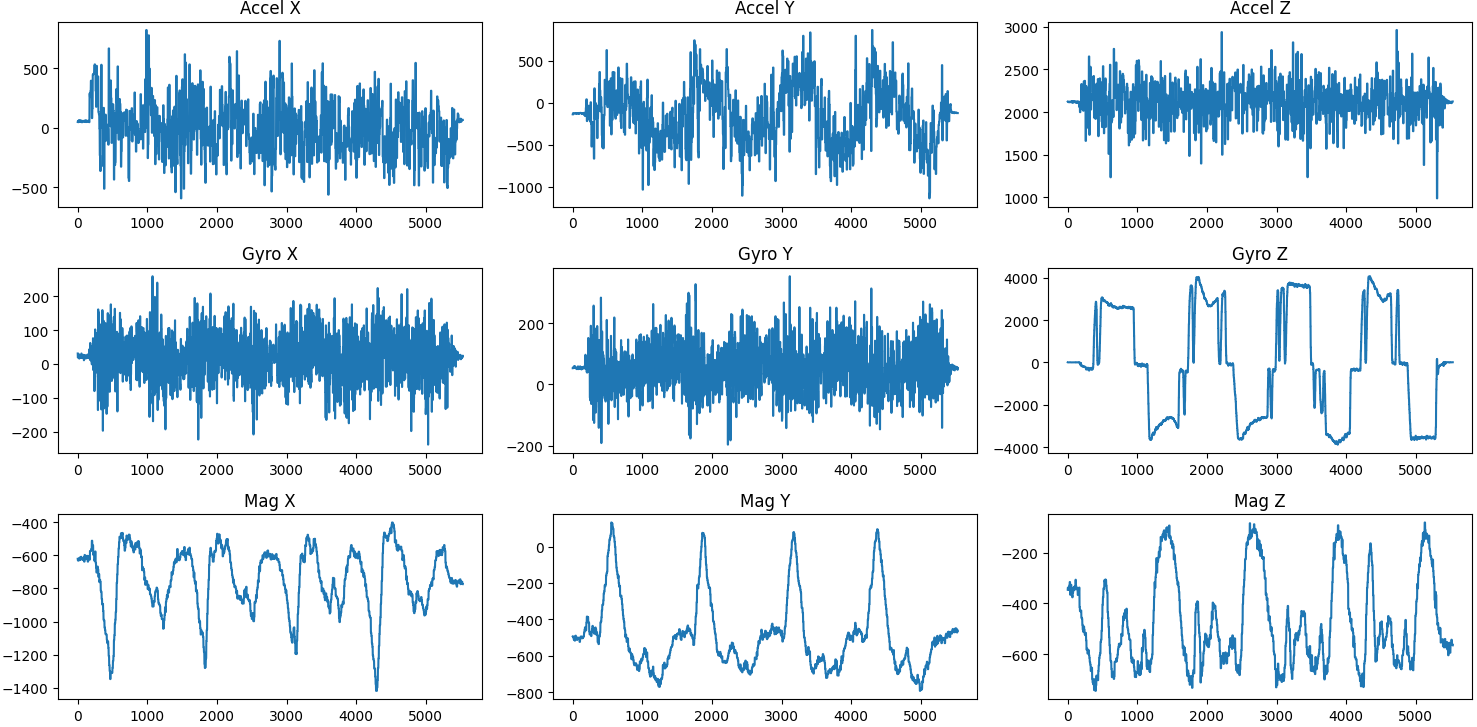
\includegraphics[width = 0.5\linewidth]{Figures/Sensors.png}
    \caption{Sensors data.}
    \label{fig:Sensors}
\end{figure}

Z analyzovaného obrázku je zřejmé, že otáčení vozidla koresponduje s daty získanými z akcelerometru na 
ose $y$ a gyroskopu na ose $z$. Nicméně je třeba poznamenat, že data z akcelerometru obsahují významný 
šum, což vyžaduje implementaci vhodného filtračního algoritmu před dalším zpracováním těchto dat. Dále 
je třeba zmínit, že data z magnetometru nelze v tomto případě využít, jelikož jsou negativně ovlivněna 
působením motoru vozidla. Možnost přesunutí senzoru magnetometru na méně náchylné místo, například 
blíže ke kameře, by byla ideální, avšak v dané konfiguraci vozidla není realizovatelná. Vzhledem k 
těmto omezením a za účelem optimalizace rychlosti zpracování bude v práci použita kombinace dat pouze z 
akcelerometru a gyroskopu.

\endinput
